%%
%%  Department of Electrical, Electronic and Computer Engineering.
%%  EPR400/2 Final Report - Section 4.
%%  Copyright (C) 2011-2021 University of Pretoria.
%%

\section{Results}

\subsection{Summary of results achieved}
\begin{table}[H]
  \centering
  \begin{tabularx}{\textwidth}{|X|X|l|}
    \hline
    \textbf{Intended outcome}                                                                                                                                                    &
    \textbf{Actual outcome}                                                                                                                                                      &
    \textbf{Location in report}                                                                                                                                                                                                                                                                                                                            \\
    \hline
    \multicolumn{3}{|l|}{\textbf{Core mission requirements and specifications}}                                                                                                                                                                                                                                                                            \\
    \hline
    The system must track mosquitoes in a mosquito enclosure and illuminate a mosquito every 5 seconds.                                                                          &
    The system tracks mosquitoes in the enclosure and illuminates a mosquito when it is stationary or moves predictably.                                                         &
    Section 4.2.1                                                                                                                                                                                                                                                                                                                                          \\
    \hline
    The laser must be able to illuminate a set point within 2 seconds accurate to within 1 millimetre.                                                                           &
    The laser is able to illuminate set point within 2 seconds accurate to within 1 millimetre.                                                                                  &
    Section 4.2.2                                                                                                                                                                                                                                                                                                                                          \\
    \hline
    The system must be able to detect mosquitoes with a 90\% accuracy and 5\% false positive rate. The detection must be updated at least every 500 milliseconds.                & The system is able to detect mosquitoes with 90\% accuracy. The detection is updated every 500 milliseconds.                                            & Section 4.2.3 \\
    \hline
    The system must be able to track mosquitoes with 90\% accuracy of correct association between frames after 5 seconds.                                                        & The system is able to track mosquitoes with 90\% accuracy or correct association between frames.                                                        & Section 4.2.4 \\
    \hline
    \multicolumn{3}{|l|}{\textbf{Field condition requirements and specifications}}                                                                                                                                                                                                                                                                         \\
    \hline
    Mosquitoes should be in an enclosure with controlled lighting and white lining on all the sides except the front facing side. The enclosure should be at least 1 metre wide. & The enclosure has \glspl{led} to control the lighting and white lining on all the sides except the front facing side. The enclosure is 0.9 metres wide. & sec           \\
    \hline
    If mosquitoes cannot be obtained a suitable substitute will be used. The substitute will be a similar flying insect.                                                         & Mosquitoes and similar flying insects were obtained. Dead mosquitoes were also used.                                                                    & sec           \\
    \hline
  \end{tabularx}
  \caption{Summary of results achieved.}
  \label{tab:results_summary}
\end{table}

\subsection{Qualification tests}
\textbf{Qualification test 1: Test of tracking and illuminating a mosquito}\\

\textit{Objectives of the test or experiment}\\
The objective of this experiment is to determine whether the system can track and illuminate a mosquito in the mosquito enclosure. The requirement states that the system must track mosquitoes in the enclosure and illuminate a mosquito every 5 seconds.

\textit{Equipment used}\\
The Nvidia Jetson Nano was used as the embedded platform to control the system. The Raspberry Pi Camera Module V2 was used to capture the video feed. The laser turret developed for this project was used to position the laser. The mosquito enclosure, laser turret, and camera was positioned as described in \autoref{subsubsec:system_positioning}. The Nvidia Jetson Nano was connected to user peripherals for user input and output. C++ code was developed specifically to capture the results for qualification test 1.

\textit{Test setup and experimental parameters}\\
Mosquitoes were simulated with a small black dot attached to a white shafts. The shafts were inserted into the enclosure and moved by hand to mimic the motion of mosquitoes.

\textit{Results or measurements}\\
The results from three different scenarios are presented in \Cref{fig:q1_1mos_detection_10fps,fig:q1_1mos_prediction_10fps,fig:q1_2mos_prediction_10fps}. The first scenario is where the laser is set to target the detected location of the mosquito. The second scenario is where the laser is set to target the predicted location of the mosquito. In the third scenario two mosquitoes were inserted into the enclosure and the laser was set to target the predicted locations of the mosquitoes.

\begin{figure}[h]
  \centering
  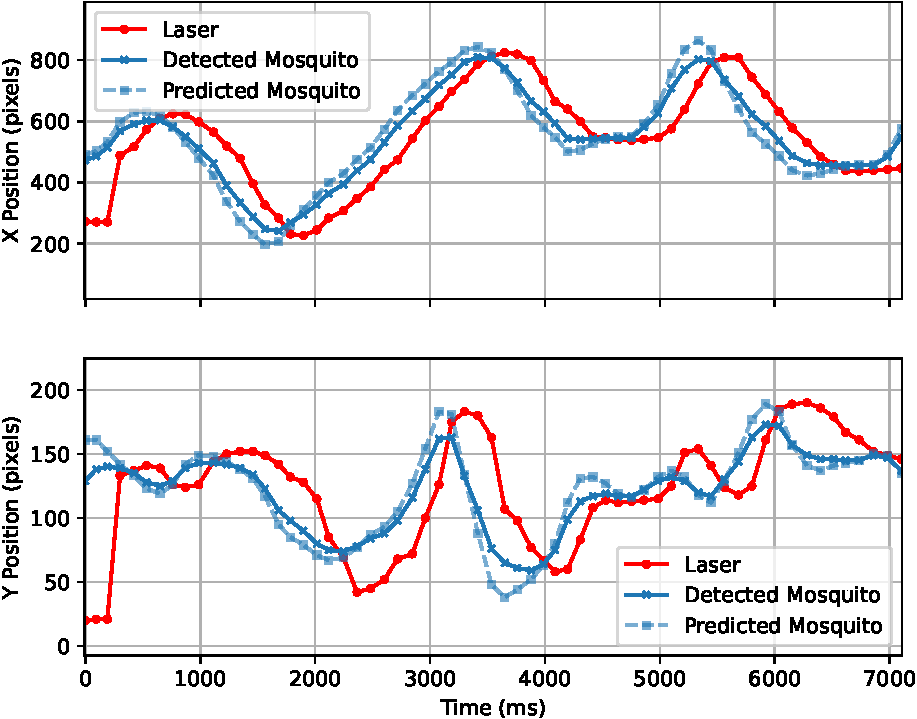
\includegraphics[width=0.8\textwidth]{figures/results/q1_1mos_detection_10fps.pdf}
  \caption{The position of the laser, detected mosquito, and predicted mosquito over time. The laser was set to target the detected location of the mosquito in this test.}
  \label{fig:q1_1mos_detection_10fps}
\end{figure}

\begin{figure}[h]
  \centering
  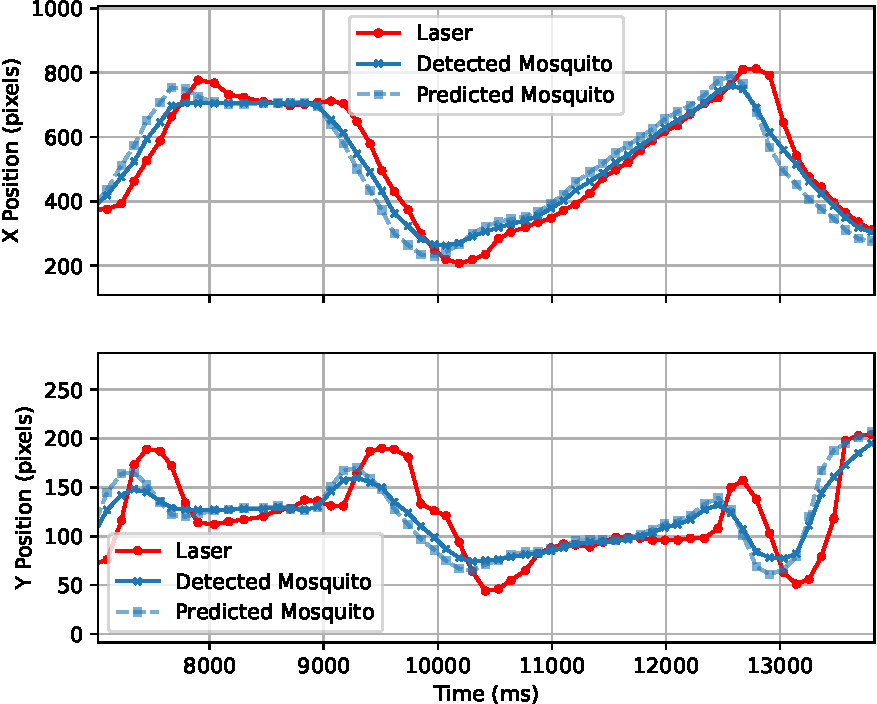
\includegraphics[width=0.8\textwidth]{figures/results/q1_1mos_prediction_10fps.pdf}
  \caption{The position of the laser, detected mosquito, and predicted mosquito over time. The laser was set to target the predicted location of the mosquito in this test.}
  \label{fig:q1_1mos_prediction_10fps}
\end{figure}

\begin{figure}[h]
  \centering
  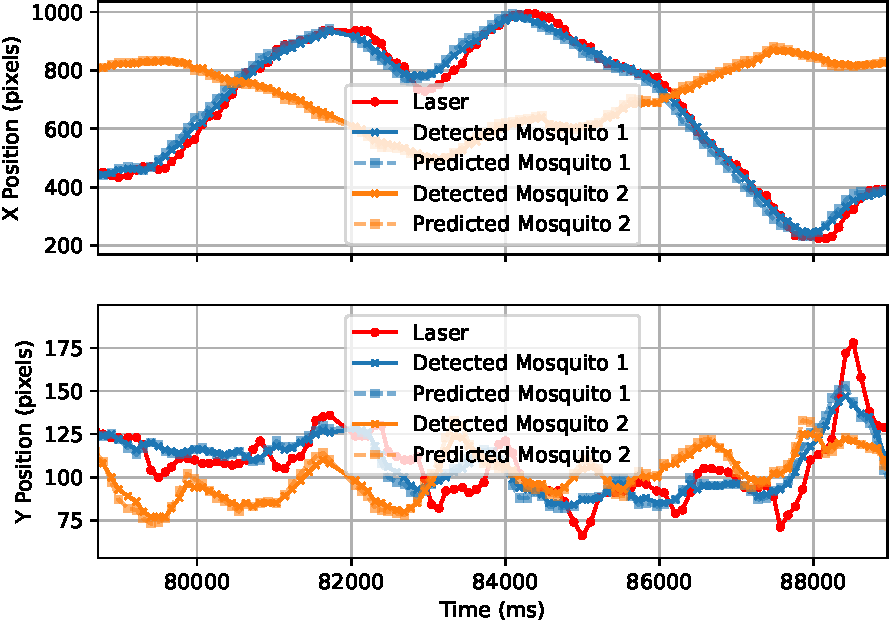
\includegraphics[width=0.95\textwidth]{figures/results/q1_2mos_prediction_10fps.pdf}
  \caption{The position of the laser, detected mosquitoes, and predicted mosquitoes with two mosquitoes in the enclosure over time. The laser was set to target the predicted location of the mosquito in this test.}
  \label{fig:q1_2mos_prediction_10fps}
\end{figure}

\textit{Observations}\\
In \Cref{fig:q1_1mos_detection_10fps,fig:q1_1mos_prediction_10fps,fig:q1_2mos_prediction_10fps}, it can be seen that the system is actively adjusting the position of the laser to track the mosquitos. In \autoref{fig:q1_1mos_detection_10fps}, the system was set to target the detected position of the mosquito. With this targeting technique it can be seen that the laser is trailing behind the actual position of the mosquito unless the mosquito is stationary. In \autoref{fig:q1_1mos_prediction_10fps}, the system was set to target the predicted position of the mosquito. With this targeting technique it can be seen that the laser reaches the actual position of the mosquito if the mosquito moves linearly for a sufficient amount of time. However, this targeting technique also results in significant overshoot when the mosquito changes direction. \autoref{fig:q1_2mos_prediction_10fps} shows the system tracking two mosquitoes in the enclosure. It can be seen that the system is able to track both mosquitoes simultaneously. The system selects one of the mosquitoes to target with the laser and the other mosquito is ignored by the laser. The same tracking behaviour is observed as in \autoref{fig:q1_1mos_prediction_10fps}, where the laser is set to target the predicted location of the mosquito.

\FloatBarrier
\textbf{Qualification test 2: Measurement of the time taken for the laser to reach a set point}\\

\textit{Objectives of the test or experiment}\\
The objective of this experiment is to measure the time it takes for the laser to reach a set point. The requirement states that the laser must be able to illuminate a set point within 2 seconds accurate to within 1 millimetre.

\textit{Equipment used}\\
The Nvidia Jetson Nano was used as the embedded platform to control the system. The Raspberry Pi Camera Module V2 was used to capture the video feed. The laser turret developed for this project was used to position the laser. The mosquito enclosure, laser turret, and camera was positioned as described in \autoref{subsubsec:system_positioning}. The Nvidia Jetson Nano was connected to user peripherals for user input and output. C++ code was developed specifically to capture the results for qualification test 2.

\textit{Test setup and experimental parameters}
\begin{enumerate}
  \item The set point was set to an arbitrary location in the mosquito enclosure.
  \item The laser was manually positioned to an arbitrary location in the mosquito enclosure.
  \item The laser turret control system was activated.
  \item The time and position of the laser was recorded for each frame captured by the system until the laser reached a settling point.
  \item Steps 1 to 4 were repeated.
\end{enumerate}

\textit{Results or measurements}\\
\autoref{fig:q2_laser_to_setpoint} shows the position of the laser over time for multiple runs with different starting points with a constant set point. \autoref{fig:q2_laser_errors} shows the euclidean distance between the laser and the set point in pixels for multiple runs with different starting points and set points. \autoref{fig:q2_laser_errors} has been restricted to the time range of 1200 to 2200 milliseconds such that the exact error between laser and set point can be observed. The radius of the laser was measured to a minimum of 5 pixels. The radius of a 1 millimetre disc was measured to be an average 2 pixels.

\begin{figure}[h]
  \centering
  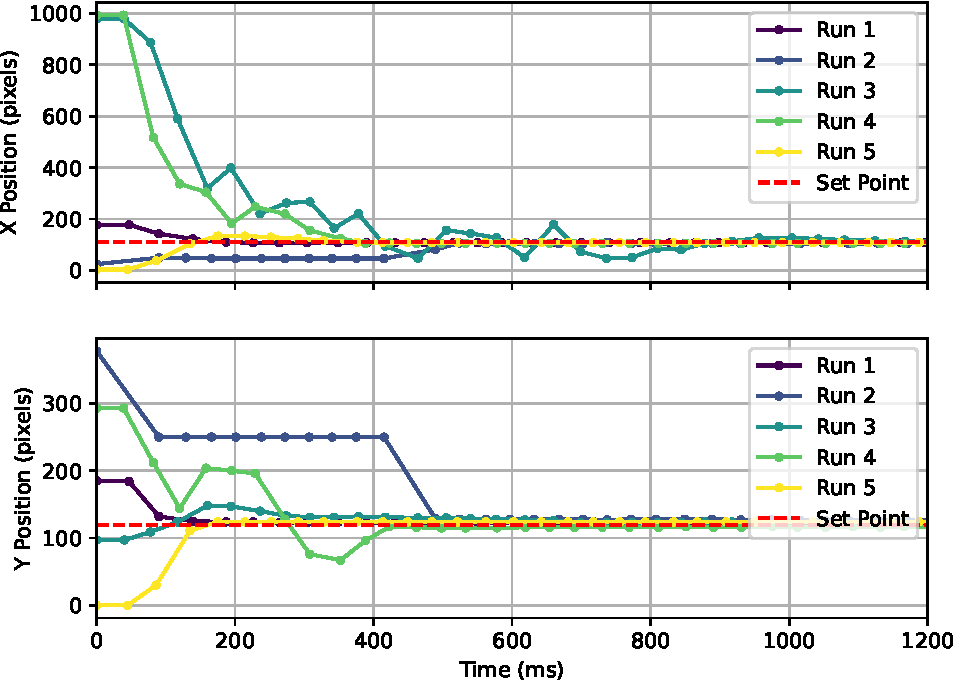
\includegraphics[width=\textwidth]{figures/results/q2.pdf}
  \caption{The position of the laser over time for multiple runs with different starting points with a constant set point.}
  \label{fig:q2_laser_to_setpoint}
\end{figure}

\begin{figure}[h]
  \centering
  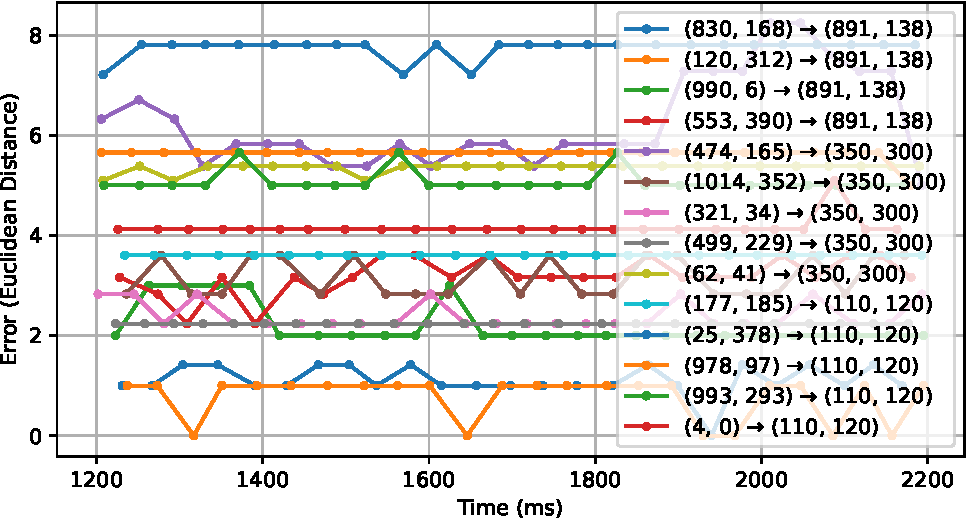
\includegraphics[width=\textwidth]{figures/results/q2_errors.pdf}
  \caption{The euclidean distance between the laser and the set point in pixels for multiple runs with different starting points and set points.}
  \label{fig:q2_laser_errors}
\end{figure}

\textit{Observations}\\
\autoref{fig:q2_laser_to_setpoint} shows the position of the laser over time for multiple runs with different starting points with a constant set point. It can be seen that general behaviour of the control system adjusts the position of the laser to move towards the set point. \autoref{fig:q2_laser_errors} shows the euclidean distance between the laser and the set point in pixels for multiple runs with different starting points and set points. The graph is restricted to the time range of 1200 to 2200 milliseconds which is after the position of the laser has stabilised. It can be seen from the various tests that the maximum euclidean distance between the laser and the set point is less the 8 pixels.

\FloatBarrier
\textbf{Qualification test 3: Test of mosquito detection}\\

\textit{Objectives of the test or experiment}\\
The objective of this experiment is to determine whether the system can detect mosquitoes in the mosquito enclosure. The requirement states that the system must be able to detect mosquitoes with a 90\% accuracy and 5\% false positive rate. The detection must be updated at least every 500 milliseconds.

\textit{Equipment used}\\
The Nvidia Jetson Nano was used as the embedded platform to control the system. The Raspberry Pi Camera Module V2 was used to capture the video feed. The laser turret developed for this project was used to position the laser. The mosquito enclosure, laser turret, and camera was positioned as described in \autoref{subsubsec:system_positioning}. The Nvidia Jetson Nano was connected to user peripherals for user input and output. C++ code was developed specifically to capture the results for qualification test 3.

\textit{Test setup and experimental parameters}\\
Mosquitoes and similar flying insect specimens were glued to white shafts as shown in \autoref{fig:dead_mossies}.
\begin{figure}
  \centering
  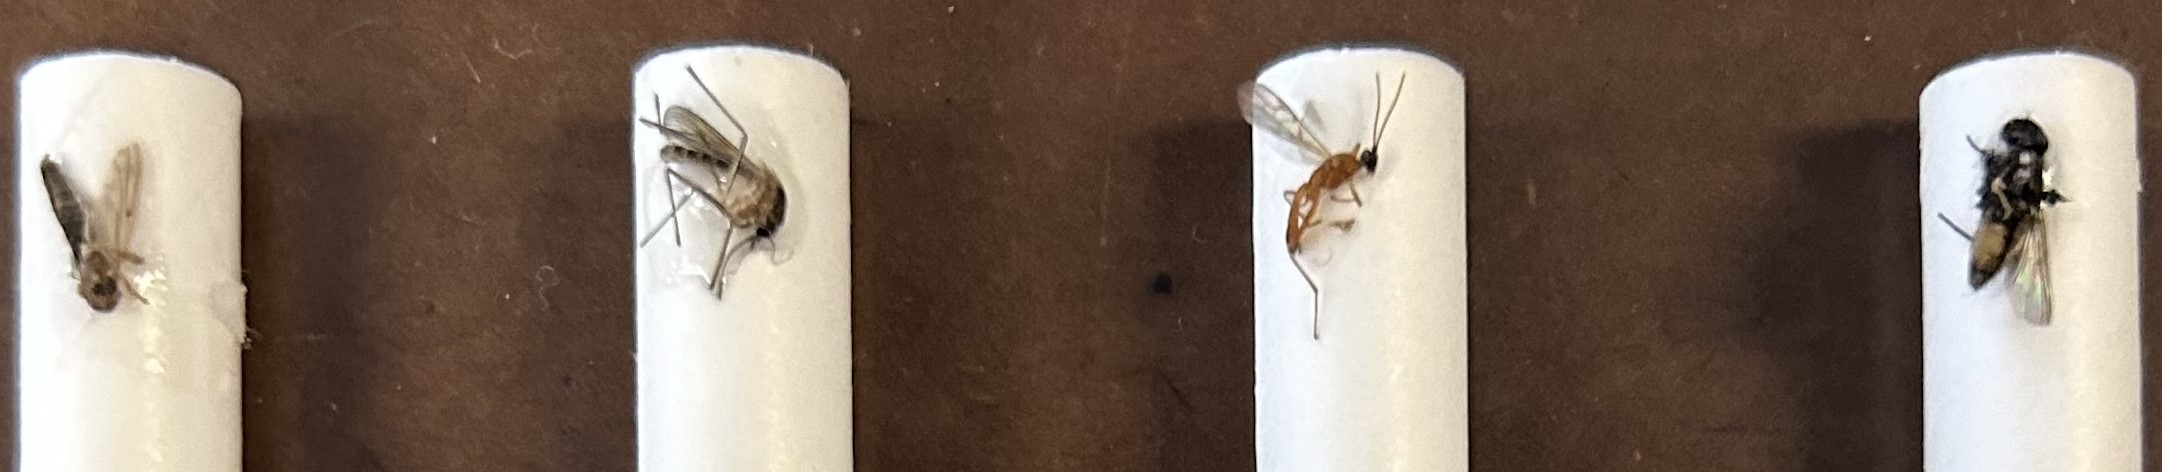
\includegraphics[width=0.8\textwidth]{figures/results/dead_mossies.jpg}
  \caption{Dead mosquitoes glued to white shafts.}
  \label{fig:dead_mossies}
\end{figure}

The test procedure was as follows:
\begin{enumerate}
  \item A known number of mosquitoes were inserted into the enclosure.
  \item The detection system was activated for 100 frames.
  \item The number of mosquitoes detected in each frame was recorded as well as the time between each frame.
  \item The experiment was repeated for different amounts of mosquitoes in the enclosure.
\end{enumerate}

\textit{Results or measurements}\\
The detection accuracy and false positive rate was determined using
\begin{equation}
  \text{Accuracy} = \frac{\text{TP} + \text{TN}}{\text{TP} + \text{TN} + \text{FP} + \text{FN}}\,,
\end{equation}
and
\begin{equation}
  \text{False positive rate (FPR)} = \frac{\text{FP}}{\text{FP} + \text{TN}}\,,
\end{equation}

where TP is the number of true positives, TN is the number of true negatives, FP is the number of false positives, and FN is the number of false negatives. The detection time requirement was determined by calculating the time between each frame.

The true positives, false positives, false negatives, and true negatives are shown in \autoref{fig:detection}. The detection update interval is shown in \autoref{fig:detection_frequency}.
\begin{figure}[h]
  \centering
  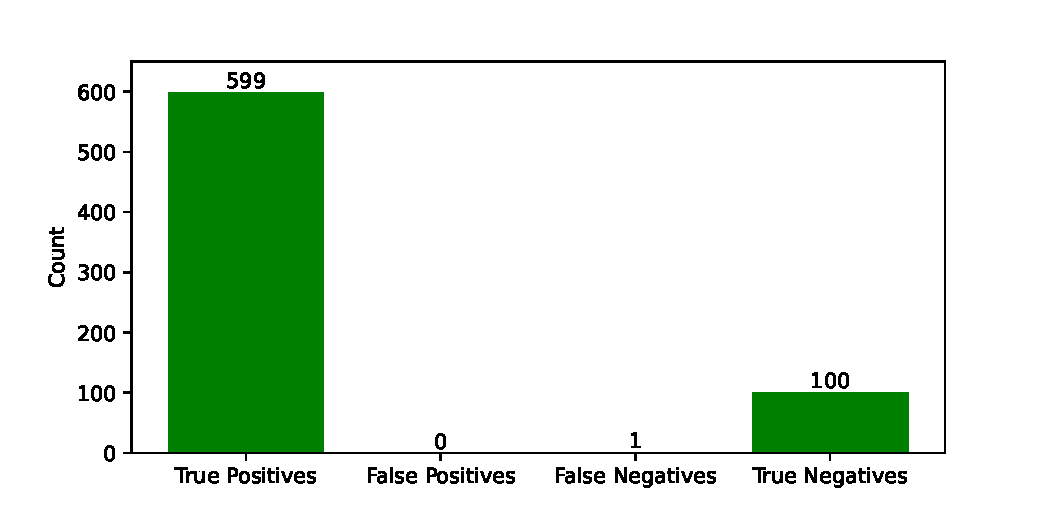
\includegraphics[width=\textwidth]{figures/results/detection.pdf}
  \caption{Mosquito detections.}
  \label{fig:detection}
\end{figure}
\begin{figure}[h]
  \centering
  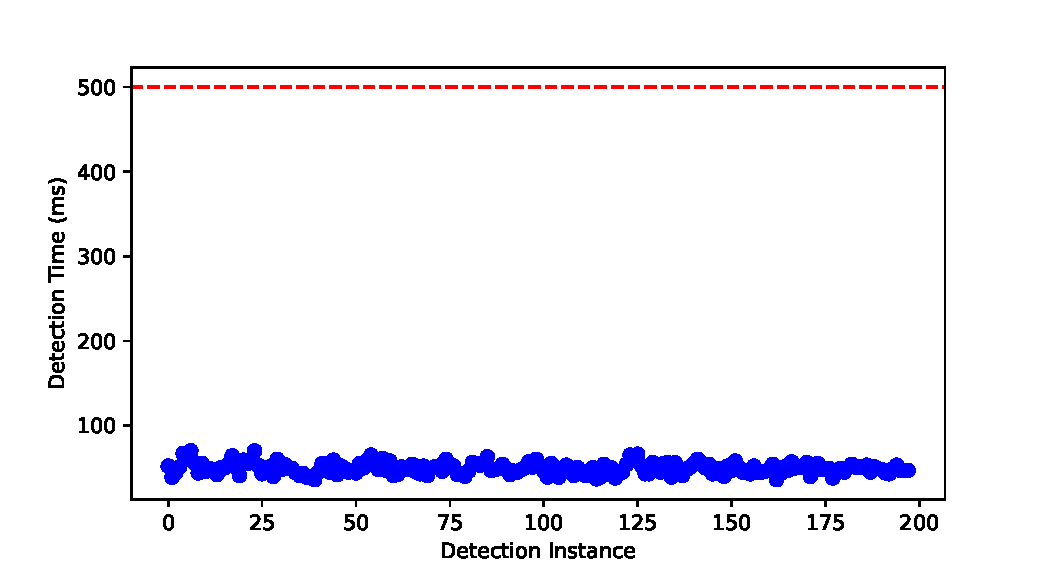
\includegraphics[width=\textwidth]{figures/results/detection_frequency.pdf}
  \caption{Mosquito detection update interval.}
  \label{fig:detection_frequency}
\end{figure}
The detection results for qualification test 3 are summarised in \autoref{tab:detection_results}
\begin{table}[h]
  \centering
  \begin{tabular}{|l|l|}
    \hline
    \textbf{Metric}                & \textbf{Value} \\
    \hline
    True Positives                 & 101            \\
    False Positives                & 0              \\
    False Negatives                & 1              \\
    True Negatives                 & 100            \\
    Accuracy                       & 0.99505        \\
    False Positive Rate            & 0.0            \\
    Detection Time Requirement Met & True           \\
    \hline
  \end{tabular}
  \caption{A summary of the detection results.}
  \label{tab:detection_results}
\end{table}

\textit{Observations}\\
The system performs detections within 100 milliseconds which is well within the 500 millisecond requirement. The system is able to detect mosquitoes with a 90\% accuracy and 5\% false positive rate.

\FloatBarrier
\textbf{Qualification test 4: Test of mosquito tracking}\label[section]{sec:tracking_quali}\\
\textit{Objectives of the test or experiment}\\
The objective of this experiment is to determine whether the system can track mosquitoes in the mosquito enclosure. The requirement states that the system must track mosquitoes in the enclosure with 90\% accuracy after 5 seconds.

\textit{Equipment used}\\
The Nvidia Jetson Nano was used as the embedded platform to control the system. The Raspberry Pi Camera Module V2 was used to capture the video feed. The laser turret developed for this project was used to position the laser. The mosquito enclosure, laser turret, and camera was positioned as described in \autoref{subsubsec:system_positioning}. The Nvidia Jetson Nano was connected to user peripherals for user input and output. C++ code was developed specifically to capture the results for qualification test 4.

\textit{Test setup and experimental parameters}\\
Mosquitoes were simulated with a small black dot attached to a white shafts.

\begin{enumerate}
  \item The mosquito shafts were inserted into the enclosure.
  \item The data capturing procedure was started.
  \item The mosquito moved by hand to mimic the motion of mosquitoes.
  \item The data capturing procedure automatically stops after 100 frames have been recorded.
\end{enumerate}

\textit{Results or measurements}\\
\autoref{fig:q4_tracking} shows the detected and predicted position of the tracked mosquitoes in the camera pixel co-ordinate system.
\begin{figure}[h]
  \centering
  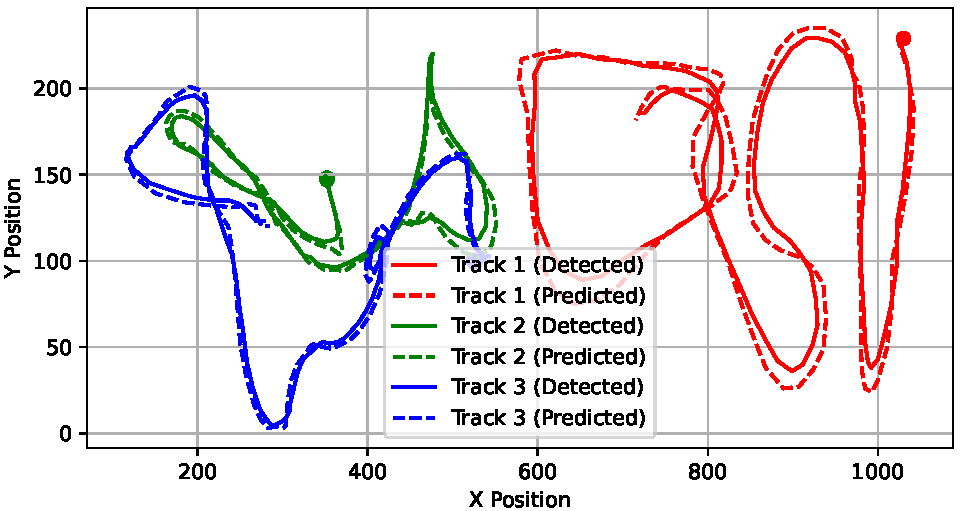
\includegraphics[width=\textwidth]{figures/results/tracking.pdf}
  \caption{The detected and predicted position of the tracked mosquitoes in the camera pixel co-ordinate system.}
  \label{fig:q4_tracking}
\end{figure}

\textit{Observations}\\
In \autoref{fig:q4_tracking}, it can be seen that the system is able correctly associate the mosquitoes between frames. The detected and predicted paths travelled by the mosquitoes are plotted. It can be seen that the predicted locations significantly deviates from the detected locations when there is a change in the direction of the path travelled by the mosquito. Three mosquitoes were tracked in this test.

\newpage

%% End of File.


